\chapter{Mode~S meteorological services}

In the current Mode~S design, two message formats are used for aircraft to communicate meteorological conditions. These messages are meteorological routine air report (MRAR) and meteorological hazard report (MHR). In this chapter, we focus on explaining the information contained in these two types of messages.

\section{Meteorological routine air report (BDS 4,4)}

In MRAR messages, information on wind, air temperature, pressure, and humidity is transmitted. The structure of the message is shown in Table \ref{tb:bds44}.


\begin{table}[ht]
\renewcommand{\arraystretch}{1.1}
\centering
\caption{Meteorological routine air report (BDS 4,4), MB field}
\label{tb:bds44}
\begin{tabular}{|l|l|l|l|}
\hline
\textbf{FIELD} & \textbf{MSG} & \textbf{MB} & \textbf{BITS} \\ \hline
Figure of merit / source & 33--36 & 1--4 & 4 \\ \hline
Status (for wind) & 37 & 5 & 1 \\ \cdashline{1-4}
Wind speed & 38--46 & 6--14 & 9 \\
~~Range: {[}0, 511{]} knots &&& \\ 
~~LSB: 1 knots &&& \\ \cdashline{1-4}
Wind direction & 47--55 & 15--23 & 9\\
~~Range: {[}0, 360{]} degrees &&& \\
~~LSB: 180/256 degrees &&& \\ \hline
Sign (for temperature) & 56 & 24 & 1 \\ \cdashline{1-4}
Static air temperature & 57--66 & 25--34 & 10\\
~~Range: {[}-128, +128{]} $^\circ$C &&& \\
~~LSB: 0.25 $^\circ$C &&& \\ \hline
Status (for pressure) & 67 & 35 & 1 \\ \cdashline{1-4}
Average static pressure & 68--78 & 36--46 & 11 \\
~~Range: {[}0, 2048{]} hPa &&& \\
~~LSB: 1 hPa &&& \\ \hline
Status (for turbulence) & 79 & 47 & 1 \\ \cdashline{1-4}
Turbulence & 80--81 & 48--49 & 2 \\ \hline
Status (for humidity) & 82 & 50 & 1 \\ \cdashline{1-4}
Humidity & 83--88 & 51--56 & 6 \\
~~Range: {[}0\%, 100\%{]} &&& \\
~~LSB: 100/64 \% &&& \\ \hline
\end{tabular}
\end{table}

The first field of the message defined the figure of merit (FOM)/source of the information. The values indicate the following:
\begin{itemize}
    \item 0: Invalid
    \item 1: Inertial system (INS)
    \item 2: Global Navigation Satellite System (GNSS)
    \item 3: Distance measuring equipment-based navigation (DME/DME)
    \item 4: Very High Frequency omnidirectional range/distance measuring equipment based navigation (VOR/DME)
    \item 5--15: Reserved
\end{itemize}

For static air temperature, the encoded value can be negative. Hence, two's complement coding (see section \ref{sec:two_complement}) is used for encoding the value. The actual maximum range of temperature is from -80 $^\circ$C to +60 $^\circ$C.

It is also worth pointing out a discrepancy in the design. The temperature is encoded using 10 bits, where the least significant bit value should have been 0.125$^\circ$. However, according to the official document \cite{icao9871v1}, the LSB value is 0.25$^\circ$. ICAO is planning to update this to 0.125$^\circ$ in the future. However, most current implementations still use 0.25$^\circ$. 

Figure \ref{fig:bds44_example} shows the decoding of an MRAR example message.

\begin{figure}[ht]
    \centering
    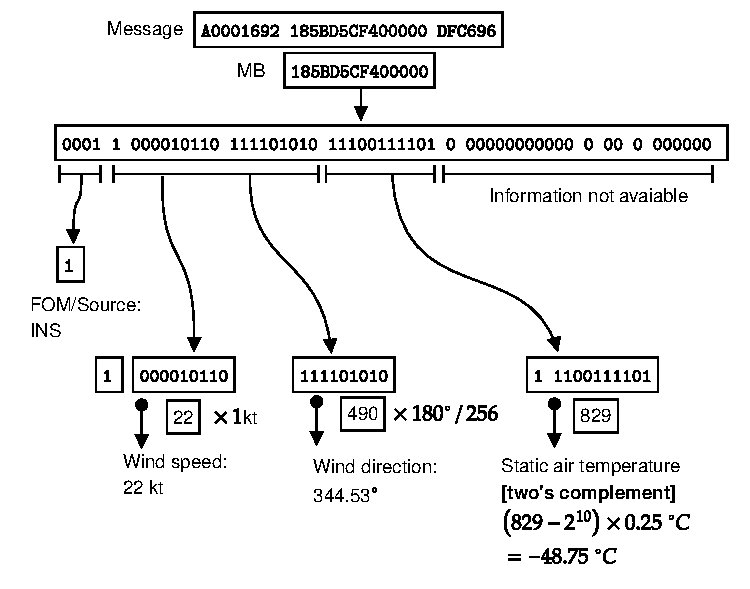
\includegraphics[scale=0.9]{figures/mode_s/bds44_example.pdf}
    \caption{Meteorological routine air report (BDS 4,4) decoding example}
    \label{fig:bds44_example}
  \end{figure}
  
\begin{notebox}{Try it out}
Using pyModeS, we can decode information of BDS 4,4 messages as: 

\begin{verbatim}
import pyModeS as pms

msg = "A0001692185BD5CF400000DFC696"

pms.commb.wind44(msg)   # (22, 344.5)
pms.commb.temp44(msg)   # (-48.75, -24.375)
pms.commb.p44(msg)      # None
pms.commb.hum44(msg)    # None
\end{verbatim}

\end{notebox}

\clearpage
\section{Meteorological hazard report (BDS 4,5)}

In MHR messages, different hazard condition levels are reported, such as turbulence, wind shear, microburst, icing, and wake vortex. It also includes temperature, pressure, and radio height. Table \ref{tb:bds45} shows the structure of the MHR message.

It is worth noting that during real flights, MHR messages are much rarer than MARA messages. Based on the tests I conducted, whenever MRAR messages are detected, most of the them only contain temperature information.

\begin{table}[ht]
\renewcommand{\arraystretch}{1.1}
\centering
\caption{Meteorological harzard report (BDS 4,5), MB field}
\label{tb:bds45}
\begin{tabular}{|l|l|l|l|}
\hline
\textbf{FIELD} & \textbf{MSG} & \textbf{MB} & \textbf{BITS} \\ \hline
Status (for turbulence) & 33 & 1 & 1 \\ \cdashline{1-4}
Turbulence & 34--35 & 2--3 & 2 \\ \hline
Status (for wind shear) & 36 & 4 & 1 \\ \cdashline{1-4}
Wind shear & 37--38 & 5--6 & 2 \\ \hline
Status (for microburst) & 39 & 7 & 1 \\ \cdashline{1-4}
Microburst & 40--41 & 8--9 & 2 \\ \hline
Status (for icing) & 42 & 10 & 1 \\ \cdashline{1-4}
Icing & 43--44 & 11--12 & 2 \\ \hline
Status (for wake vortex) & 45 & 13 & 1 \\ \cdashline{1-4}
Wake vortex & 46--47 & 14--15 & 2 \\ \hline
Status (for temperature) & 48 & 16 & 1 \\ \cdashline{1-4}
Sign (for temperature) & 49 & 17 & 1 \\ \cdashline{1-4}
Static air temperature & 50--58 & 18--26 & 9 \\
~~Range: {[}-128, +128{]} $^\circ$C &&& \\
~~LSB: 0.25 $^\circ$C &&& \\ \hline
Status (for pressure) & 59 & 27 & 1 \\ \cdashline{1-4}
Average static pressure & 60--70 & 28--38 & 11\\
~~Range: {[}0, 2048{]} hPa &&& \\
~~LSB: 1 hPa &&&  \\ \hline
Status (for height) & 71 & 39 & 1 \\ \cdashline{1-4}
Radio height & 72--83 & 40--51 & 12 \\
~~Range: {[}0, 65 528{]} ft &&& \\
~~LSB: 16 ft &&& \\ \hline
Reserved & 84--88 & 52--56 & 5 \\ \hline
\end{tabular}
\end{table}

The levels for turbulence, wind shear, microburst, icing, and wake vortex are encoded as follows:
\begin{itemize}
  \item \texttt{00}: NIL
  \item \texttt{01}: LIGHT
  \item \texttt{10}: MODERATE
  \item \texttt{11}: SEVERE
\end{itemize}

As is the case for MRAR messages, the actual range of the temperature is from -80 $^\circ$C to +60 $^\circ$C, and it is encoded using the two's complement coding.

Figure \ref{fig:bds45_example} shows the decoding of an example message. Note that in this example, only the air temperature information is included. None of the hazard conditions is reported.

\begin{figure}[ht]
  \centering
  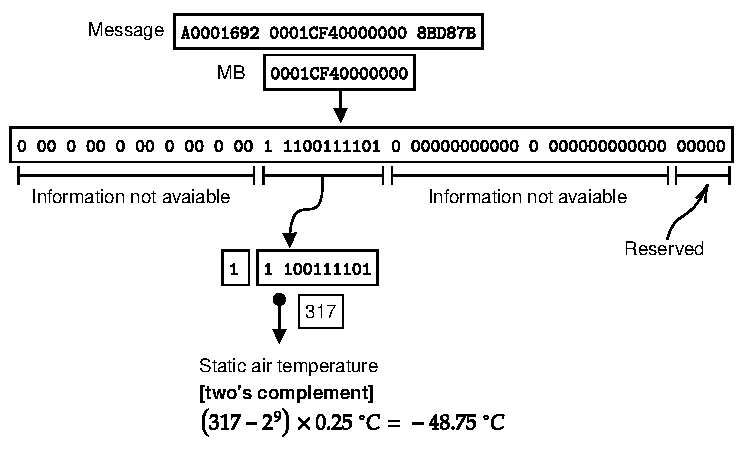
\includegraphics[scale=0.9]{figures/mode_s/bds45_example.pdf}
  \caption{Meteorological harzard report (BDS 4,5) decoding example}
  \label{fig:bds45_example}
\end{figure}


\begin{notebox}{Note}
The availability of BDS 4,4 messages is quite low. Very few aircraft's transponders have these capabilities enabled. BDS 4,5 messages are even rarer. When such a message is transmitted, it is very common that the information in many fields is not available.
\end{notebox}

